% LEGO Analytics Engineer — Case Study Report
% Compile: pdflatex -interaction=nonstopmode LEGO_Case_Study_Report.tex (run twice for TOC/refs)
\documentclass[11pt,a4paper]{article}

\usepackage[utf8]{inputenc}
\usepackage[T1]{fontenc}
\usepackage{lmodern}
\usepackage[margin=22mm]{geometry}
\usepackage{microtype}
\usepackage{graphicx}
\usepackage{xcolor}
\usepackage{booktabs}
\usepackage{array}
\usepackage{hyperref}
\usepackage{tikz}
\usetikzlibrary{shapes.geometric, arrows.meta, positioning, calc, fit, backgrounds}

% --- Job-description keyword highlighting (tailored to Innovation & Automation / Analytics & Insights) ---
\definecolor{KwFill}{RGB}{255,243,200}
\definecolor{KwFrame}{RGB}{200,120,0}
\definecolor{LegoRed}{RGB}{227,0,11}
\newcommand{\JD}[1]{\colorbox{KwFill}{\textbf{\small #1}}}

\hypersetup{
  colorlinks=true,
  linkcolor=LegoRed,
  urlcolor=LegoRed,
  citecolor=LegoRed,
}

\title{\textbf{Evaluation \& Governance for LLM Campaign Assistants}\\[0.4em]
\large A portfolio release-gate MVP aligned with Analytics Engineering practice}
\author{Case study (job application)}
\date{\today}

\begin{document}
\maketitle

\begin{abstract}
\noindent
This report describes a small but production-aware system for \JD{evaluation frameworks}, \JD{observability}, and \JD{AI governance} applied to \JD{LLM}-generated campaign recommendations---a use case adjacent to \JD{campaign optimisation} and commercial decision support. The artefact demonstrates \JD{regression-style} comparison between \JD{baseline} and \JD{candidate} prompt versions, \JD{quality gates}, sample-size-aware stability checks, and \JD{segmented evaluation} to avoid \JD{hidden regressions} when a change looks good on narrow examples but fails \JD{portfolio-wide}.
\end{abstract}

\section{Role alignment (Innovation \& Automation, Analytics \& Insights)}
The target role emphasises building systems that make \JD{reliability an engineering discipline}, not a compliance exercise: \JD{evaluation frameworks for LLM and agent outputs}, \JD{structured regression suites}, \JD{human-in-the-loop review} where ground-truth labels are incomplete, and \JD{observability} linking model behaviour to \JD{business outcomes}. It also values strong \JD{Python engineering}, \JD{SQL}, \JD{REST API} consumption, \JD{lifecycle management} (deploy/monitor, not only training), collaboration with the \JD{Data Office} and \JD{Digital Product} teams, and reusable templates---with \JD{CI/CD} (\JD{GitHub Actions}) as a natural next step for hardening.

\section{Business problem (commercial context)}
Marketing and growth teams increasingly rely on internal assistants for \JD{campaign optimisation} style workflows (brief $\rightarrow$ concrete actions). The risk is not ``model quality in isolation'' but \textbf{release risk}: a new prompt can improve one scenario while silently degrading others. The question becomes:

\begin{center}
\fbox{\parbox{0.92\linewidth}{
\textbf{Is a candidate assistant version safe to deploy \emph{portfolio-wide}?}\\[0.3em]
If evaluation is only anecdotal (``it reads better''), teams ship \JD{hidden regressions} and lose trust---exactly the class of failure \JD{governance} and \JD{observability} are meant to prevent.
}}
\end{center}

\section{Process maps (business process view)}

\subsection{Where this sits: engineering vs.\ daily marketing use}
Figure~\ref{fig:twoflows} separates \textbf{daily use} of an assistant from \textbf{pre-release evaluation}---the focus of this MVP.

\begin{figure}[htbp]
\centering
\begin{tikzpicture}[
  font=\small,
  box/.style={rectangle, draw, rounded corners, align=center, minimum width=3.2cm, minimum height=0.9cm},
  arrow/.style={-{Stealth[length=2.2mm]}, thick},
]

\node[box, fill=gray!10] (m) {Marketing /\\campaign team};
\node[box, fill=blue!8, right=1.6cm of m] (a) {Internal \JD{LLM} assistant}\\(production path);
\node[box, fill=green!10, right=1.6cm of a] (o) {Campaign actions\\(briefs, creatives)};

\draw[arrow] (m) -- (a);
\draw[arrow] (a) -- (o);

\node[box, fill=orange!12, below=1.3cm of a] (e) {\textbf{Analytics / AI engineering}\\\textbf{Release evaluation (this MVP)}};
\node[box, fill=yellow!15, left=1.6cm of e] (c) {Change request:\\prompt / model / rules};
\node[box, fill=yellow!15, right=1.6cm of e] (g) {\JD{Quality gate} decision\\\texttt{PROMOTE} / \texttt{BLOCK} / conditional};

\draw[arrow] (c) -- (e);
\draw[arrow] (e) -- (g);

\draw[dashed, gray] ($(a.south west)+(-0.6,-0.25)$) rectangle ($(g.north east)+(0.6,0.25)$);
\node[anchor=north west, font=\scriptsize\itshape] at ($(a.south west)+(-0.5,-0.35)$) {Engineering control loop (offline / pre-release)};

\end{tikzpicture}
\caption{Two flows: daily assistant usage (top) vs.\ pre-release evaluation and \JD{governance} (bottom).}
\label{fig:twoflows}
\end{figure}

\subsection{End-to-end release gate (BPM-style)}
Figure~\ref{fig:gate} shows the evaluation lifecycle from change intake to a documented decision---the same structure used for \JD{lifecycle management} in production ML systems.

\begin{figure}[htbp]
\centering
\begin{tikzpicture}[
  font=\small,
  start/.style={rectangle, draw, rounded corners, fill=blue!6, minimum width=2.8cm, minimum height=0.9cm, align=center},
  step/.style={rectangle, draw, rounded corners, minimum width=2.8cm, minimum height=0.9cm, align=center},
  decision/.style={diamond, draw, aspect=2, inner sep=0.5mm, align=center, minimum width=2.8cm},
  gate/.style={rectangle, draw, rounded corners, fill=red!8, thick, minimum width=3.2cm, minimum height=1.0cm, align=center},
  arrow/.style={-{Stealth[length=2mm]}, thick},
]

\node[start] (in) {Intake:\\baseline vs.\ candidate};
\node[step, right=1.1cm of in] (ds) {Load test suite\\(\JD{regression} cases)};
\node[step, right=1.1cm of ds] (run) {Execute both versions\\(same inputs)};
\node[step, below=0.9cm of run] (sc) {Score outputs\\(rubric + checks)};
\node[step, left=1.1cm of sc] (cmp) {Aggregate + compare\\(portfolio mean)};
\node[gate, below=0.9cm of cmp] (gv) {\JD{Quality gate}\\(thresholds +\\sample-size rules)};
\node[decision, below=0.9cm of gv] (d) {Pass?};
\node[step, right=1.6cm of d] (pr) {Document decision\\\& \JD{observability} trail};
\node[step, left=1.6cm of d] (bl) {\texttt{BLOCK}\\rework candidate};

\draw[arrow] (in) -- (ds);
\draw[arrow] (ds) -- (run);
\draw[arrow] (run) -- (sc);
\draw[arrow] (sc) -- (cmp);
\draw[arrow] (cmp) -- (gv);
\draw[arrow] (gv) -- (d);
\draw[arrow] (d) -- node[above, font=\scriptsize] {yes} (pr);
\draw[arrow] (d) -- node[above, font=\scriptsize] {no} (bl);

\end{tikzpicture}
\caption{Release evaluation loop: structured regression, scoring, aggregation, and \JD{quality gates}.}
\label{fig:gate}
\end{figure}

\subsection{Segmentation: why portfolio-level gates matter}
Figure~\ref{fig:segment} summarises the key insight: a \textbf{single prompt rarely generalises} across all campaign types; \JD{segmented evaluation} makes the failure mode visible.

\begin{figure}[htbp]
\centering
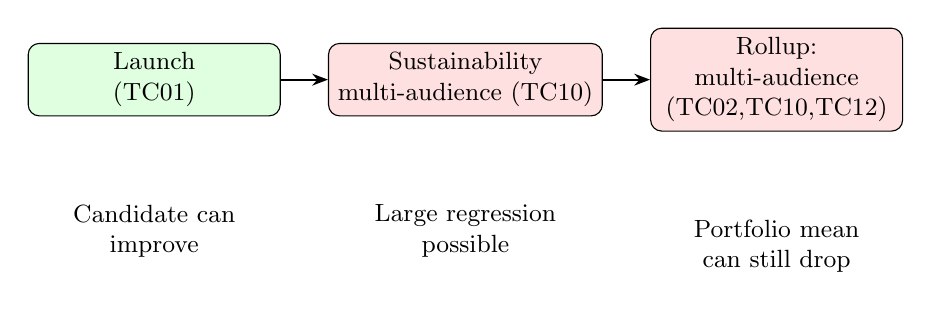
\begin{tikzpicture}[
  font=\small,
  seg/.style={rectangle, draw, rounded corners, minimum width=3.2cm, minimum height=0.85cm, align=center},
  good/.style={fill=green!12},
  bad/.style={fill=red!12},
  arrow/.style={-{Stealth[length=2mm]}, thick},
]

\node[seg, good] (l) {Launch\\(TC01)};
\node[seg, bad, right=0.6cm of l] (s) {Sustainability\\multi-audience (TC10)};
\node[seg, bad, right=0.6cm of s] (r) {Rollup:\\multi-audience\\(TC02,TC10,TC12)};

\node[below=1.0cm of l, align=center] {Candidate can\\improve};
\node[below=1.0cm of s, align=center] {Large regression\\possible};
\node[below=1.0cm of r, align=center] {Portfolio mean\\can still drop};

\draw[arrow] (l) -- (s);
\draw[arrow] (s) -- (r);

\end{tikzpicture}
\caption{Illustrative segmentation story: local wins do not imply global safety.}
\label{fig:segment}
\end{figure}

\section{What was built (technical summary, aligned to role)}
\begin{itemize}
  \item \textbf{Language/runtime:} \JD{Python} implementation, SQLite storage for \JD{analytical datasets} and run history, \JD{REST API} calls to a hosted LLM for generation and judging.
  \item \textbf{Evaluation:} rubric + deterministic checks; baseline vs.\ candidate \JD{regression}; per-case and portfolio aggregates.
  \item \textbf{Governance:} \JD{quality gates} with explicit decisions; sample-size-aware variance gating; \texttt{PROMOTE\_CONDITIONAL} when confidence is low.
  \item \textbf{Observability:} historical run reports and trend-style summaries (Phase 4 style), plus segmented tables.
  \item \textbf{Reusability:} prompt versions as configuration; suite files as \JD{benchmarks}; scripts as repeatable entrypoints.
\end{itemize}

\section{Results (validation suite, $n=8$)}
Reference runs: baseline \textbf{21}, candidate \textbf{22}. Portfolio gate outcome: \textbf{\texttt{BLOCK}} with high confidence ($n\ge 5$ for stability checks).

\begin{table}[htbp]
\centering
\small
\begin{tabular}{@{}lrrr@{}}
\toprule
\textbf{Metric (mean)} & \textbf{Baseline} & \textbf{Candidate} & \textbf{$\Delta$} \\
\midrule
Relevance & 2.966 & 2.901 & $-0.065$ \\
Actionability & 4.750 & 4.300 & $-0.450$ \\
Constraints & 7.501 & 7.085 & $-0.416$ \\
Structure & 4.165 & 3.955 & $-0.210$ \\
\textbf{Aggregate} & \textbf{4.844} & \textbf{4.542} & \textbf{$-0.302$} \\
\bottomrule
\end{tabular}
\caption{Portfolio mean scorecard (illustrative scoring scale 0--10).}
\end{table}

\subsection{Segmented signals (rollup)}
\begin{table}[htbp]
\centering
\small
\begin{tabular}{@{}lrrr@{}}
\toprule
\textbf{Group} & \textbf{Mean $\Delta$ aggregate} & \textbf{Signal} & \textbf{Notes} \\
\midrule
Launch (TC01) & $+1.250$ & PROMOTE\_SEGMENT & structured launch brief \\
Sustainability (TC10) & $-3.462$ & BLOCK\_SEGMENT & multi-audience + channels \\
Multi-audience rollup (TC02, TC10, TC12) & $-1.043$ & BLOCK\_SEGMENT & generalisation failure \\
\bottomrule
\end{tabular}
\caption{Segmentation explains \emph{where} a candidate improves vs.\ fails.}
\end{table}

\section{Final decision story (executive)}
\textbf{Question:} Is candidate v3 safe to deploy globally?\\
\textbf{Answer:} \textbf{No --- BLOCK.}\\
\textbf{Evidence:} portfolio mean decreased; strong regression on \JD{sustainability} / multi-audience scenario (TC10) despite gains on a launch case (TC01).\\
\textbf{Decision:} do not ship v3 as the default; consider \JD{scoped release} or routing by brief type.

\section{Future hardening (next engineering steps)}
This MVP intentionally stops before heavy platform work. Natural extensions align with the posting: \JD{GitHub Actions} for scheduled evaluation, \JD{MLflow}-style experiment tracking, \JD{Databricks}-style deployment patterns, and deeper \JD{drift detection} once production telemetry exists.

\section{Closing statement}
The core contribution is not ``a better chatbot,'' but a \textbf{control system} for \JD{LLM} assistant changes: measurable, auditable, and aligned with \JD{commercial decision} risk.

\end{document}
